\chapter{Разработка системы}
\label{cha:impl}

\section{Выбор стека технологий и решений}

Для разработки будем использовать данный стек как основу:

\begin{itemize}
    \item Операционная система: Астра Линукс - это российская операционная система на базе GNU / Linux. Астра Линукс поставляется с множеством компонентов, которые поддерживают важные функции, с помощью ядра, системные утилиты и GUI. \cite{dev:astra_linux}
    \item Компилятор: LCC 1.25.20 - это локальный C-компилятор для процессоров e2k \cite{dev:elbrus_lcc}. Это портативный компилятор для языка C с открытым исходным кодом, который поддерживается на многих архитектурах и системах.
    \item Язык программирования: Python 3.10 - это последняя версия популярного языка программирования с открытым исходным кодом. Python известен его читаемостью и лаконичностью, что делает его идеальным для разработки и автоматизации.
    \item Nginx - это мощный веб-сервер с открытым исходным кодом (и обратным прокси), который известен своей скоростью и гибкостью. Используется для обслуживания статического содержимого, балансировки нагрузки, кэширования и т.д.
    \item Эльбрус - это серия высокопроизводительных процессоров разработки российской корпорации "МЦСТ". \cite{dev:elbrus_cpu}
    \item СУБД: PostgreSQL Pro.
    \item Инструменты контейнеризации: Такие инструменты как Docker могут понадобиться для контейнеризации нашей системы и управления ими с целью упрощения развертывания, масштабирования и работы в рамках микросервисной архитектуры.

\Define{СУБД}{Система управления базами данных}

\end{itemize}

На стороне серверной части будет использоваться фреймворк Flask, для создания и обслуживания API, через которое клиенты могут взаимодействовать с системой. Flask позволяет быстро и эффективно разрабатывать веб-приложения благодаря своему легкому и гибкому коду. 

Для обработки и хранения данных будет использоваться реляционная база данных PostgreSQL, которая известна своей надежностью, мощностью и поддержкой обширных возможностей SQL. 

Обмен данными между клиентом и сервером будут осуществлять путем создания REST API, что позволяет клиентам отправлять запросы на сервер и получать ответы в удобном для обработки формате, таком как JSON.

Реализация серверной части будет производиться с использованием Python 3.10, что облегчит интеграцию с Flask, а также предоставит широкие возможности для ее дальнейшей разработки и оптимизации.

Для обеспечения безопасности и стабильности работы всей системы, серверная часть будет развернута в контейнерах Docker, что также упростит процесс развертывания и обновления приложения.

Весь код серверной части будет писаться с использованием стандартов PEP 8 \cite{dev:pep} для обеспечения его качества, читаемости и поддерживаемости. 

\Define{PEP}{Python Enhancement Proposal ""--- стандарт написания кода на языке Python, постановление об оформлении кода для языка Python. Этот стандарт разработал Гвидо ван Россум, основатель Python, с помощью Барри Уорсо, чтобы код был более читаемым и унифицированным.}

Наконец, для мониторинга работы сервера и отслеживания возможных ошибок и неполадок будет использоваться система логирования. 

Все эти инструменты и технологии будут работать вместе, чтобы обеспечить стабильную, эффективную и безопасную систему дистрибьюции модулей.

\section{Подготовка рабочего окружения}

\subsection{Получение сервера с Elbrus-8CV}

Отправляем запрос на доступ, чтобы получить доступ к серверу Sumireko, который находится по адресу https://elbrus.kurisa.ch/ и работает на базе Эльбрус-8СВ. Этот запрос обычно включает нашу информацию об учетной записи, такую как имя пользователя на сервере, ключ и никнейм телеграм.

Генерируем пары ключей с помощью утилиты ssh-keygen. Этот процесс включает в себя создание открытого и закрытого ключей, которые используются для защищенного подключения к серверу. 

\begin{verbatim}
ssh-keygen -t rsa -b 4096 -C "sepera_okeq@economic-crisis.com"
\end{verbatim}

После того, как мы сгенерировали ключи, мы можем отправить наш открытый ключ в заявке на доступ и зайти на сервер.

\begin{figure}
  \centering
  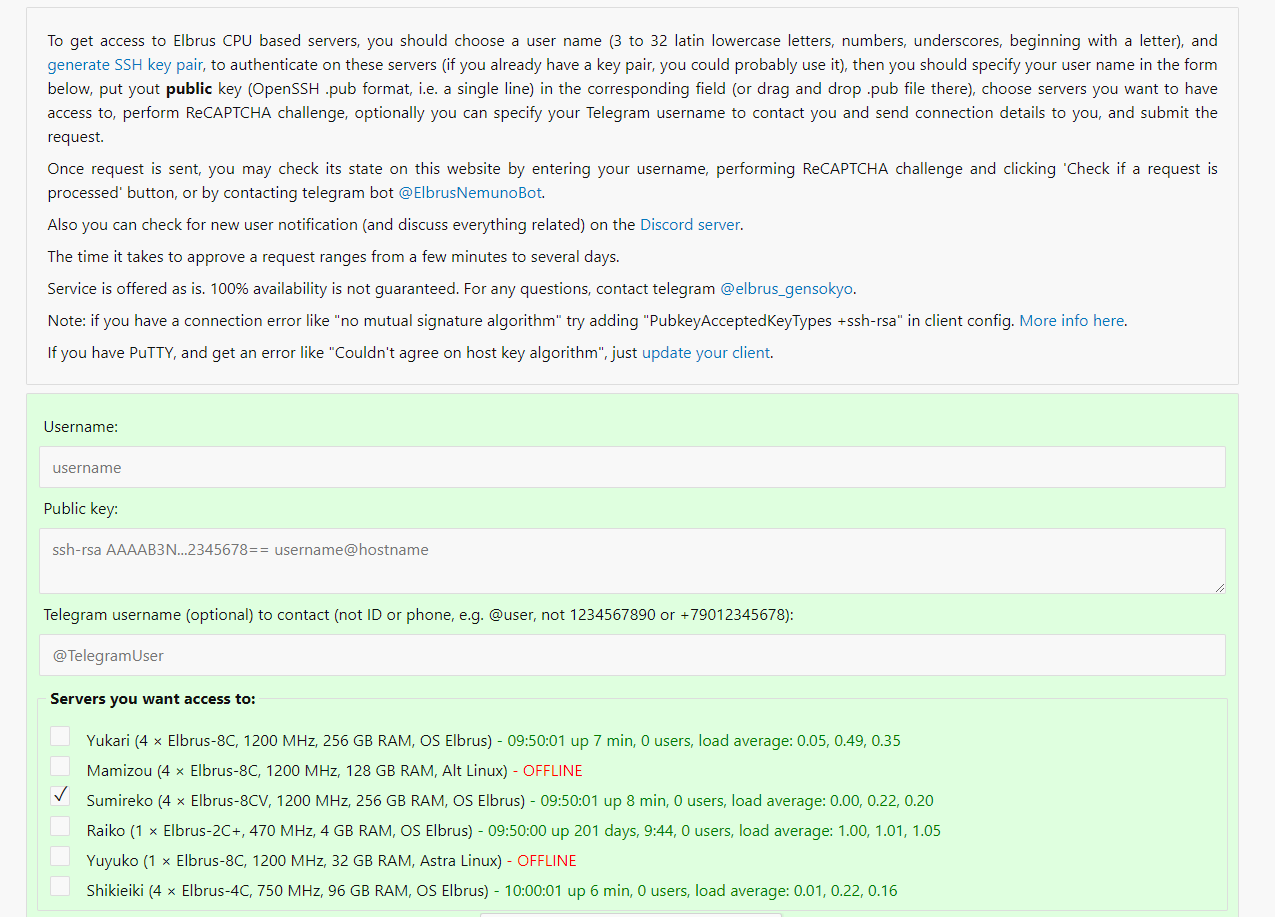
\includegraphics[width=.9\textwidth]{graphics/img/elbrus_dostyp.png}
  \caption{Получение доступа к серверу с Эльбрус-8СВ}
  \label{fig:elbrus-dostup}
\end{figure}

Для выбора сервера Sumireko мы введем его данные в наш ssh-клиент. Этот сервер имеет 4 процессора Elbrus-8CV с частотой 1200 МГц, 256 ГБ оперативной памяти и операционную систему Elbrus OS.

На сервере Sumireko мы будем развертывать виртуальный сервер KVM на основе Astra Linux. Это создаст изолированное окружение, которое мы можем использовать для различных задач.

\subsection{Сборка необходимых средств}

Для компиляции исходного кода необходимо использование компилятора LCC, доступного для получения на веб-портале МЦСТ.

Наконец, мы можем собрать Python 3.10 из исходников. Для этого мы сначала загрузим исходный код с официального веб-сайта Python, а затем выполним команды, необходимые для компиляции и установки.

\begin{listing}[H]
\cfile{../src/1}
\end{listing}
\label{lst:c}

Добавляем переменные окружения для Python:

\begin{listing}[H]
\cfile{../src/2}
\end{listing}
\label{lst:c}


Так как e2k является специфичной платформой, где нет спекулятивного механизма, который позволяет интрепртетируемым языкам и языкам с виртуальной машиной работать быстрее, то нужно пропатчить и пересобрать Python.

\begin{listing}[H]
\cfile{../src/patch_python.c}
\caption{Патч — python-patch.sh} 
\end{listing}
\label{lst:c}

Мы проводим повторную сборку и получаем доступ к скомпилированной версии Python 3.10 для e2k.

Установим средства KVM QEMU и iso образ AstraLinux c https://download.astralinux.ru/astra/stable/orel/iso/.

После установки имеется готовая и чистая виртуальная среда, которая станет полигном для нашей работы. 

\section{Конфигурация Gatawey}

Скачиваем собранную версию Nginx из репозиториев Elbrus OS, предлагаемых компанией МЦСТ.

Создадим конфигурацию настроек сервера Nginx, чтобы она поддерживала JWT и работала в связке PostgresSQL для достижения высокой производительности СУБД, из-за нативной поддержки на e2k с более высокой скоростью работы. Нам необходимо определить отдельные субдомены api, которые будет отвечать за работу с бэкенд частью и modules, являясь статичным хранилищем модулей.


\inputminted[fontsize=\small]{text}{../src/nginx}

\section{Разработка серверной части}

Используем библиотеку Flask для создания сервера, который может обрабатывать HTTP-запросы, связанные с загрузкой, хранением и передачей пакетов.

Создаем Flask приложение с использоваем flask.Flask(). 

Определяем местоположение каталога «packages», где будут храниться все пакеты (модули). Это должна быть та же папка, что и для alias, ссылающего на /path/to/modules в конфигурации Gatawey. 

\begin{listing}[H]
\cfile{../src/dev1}
\end{listing}
\label{lst:c}

Запрос «/search» ищет все совпадения через регулярное выражение, позволяющее найти вхождение в любом месте названия файла, исключая его расширение.

Определяем маршруты для запросов GET к «/packages/». Если файл по запрашиваемому пути существует, он возвращается клиенту. 

Если папки «packages» нет, она создается. В маршруте «/upload» обрабатываются POST-запросы для загрузки пакетов. При получении запроса проверяется наличие всех требуемых полей («name», «version» и файл). Если какое-либо из полей отсутствует, возвращается ошибка 400 с сообщением. 

\begin{listing}[H]
\cfile{../src/dev2} 
\end{listing}
\label{lst:c}

Загруженный пакет сохраняется в каталоге «packages», имя файла формируется из имени пакета и версии. Кроме того, проверка производится, чтобы убедиться, что загружаемый пакет является самым последним по версии. Если это так, копия загруженного пакета сохраняется как «latest». 

\begin{listing}[H]
\cfile{../src/dev3} 
\end{listing}
\label{lst:c}


Запрос «/cve» ищет все совпадения по базам БДУ и CVE, уведомляя о последних 10 открытых проблемах.


\section{Разработка клиентской части}

Определим подкоманды `install`, `search`, `uninstall` и `upload`, которые выполняют различные операции с модулями, создав обработчик команд.

Когда используется подкоманда `install`, скрипт разделяет имя пакета и его версию, указанные в аргументе. Если версия не указана, она устанавливается как «latest». Затем он проверяет наличие каталога «modules», создает его, если он отсутствует, и удаляет существующий пакет, если он уже установлен. После этого скрипт загружает пакет со специфического URL и устанавливает его в каталог «modules».

При использовании подкоманды `uninstall`, скрипт немного похож на `install`, но вместо загрузки и установки пакета он удаляет указанный пакет, если такой существует.

Подкоманда `upload` использует указанный в аргументе каталог для создания zip-архива и загрузки его на сервер. Этот процесс включает в себя чтение файла "module.json" в указанном каталоге, чтобы получить название и версию пакета, а затем отправку zip-архива и этой информации на сервер.

Подкоманда `info` отображает сведения о модуле, включая информацию о его локальной установке и другие детали.

Подкоманда `search` ищет все совпадения в названиях модулей.

Подкоманда 'cve' ищет все увязвимости в локальных пакетах, а 'cve --global' демонстрирует список увязвимостей на сервере.

\section{Упаковка в пакет для распространения}

Создадим файл pyproject.toml, который служит для описания метаданных пакета и определения того, как пакет должен быть построен. В этом файле указаны имя пакета, версия, авторы, базовые зависимости, ссылки и прочее. 

\inputminted[fontsize=\small]{text}{../src/pyproject}

%рис.~\ref{fig:spire01}
%\begin{listing}[H]
%\cfile{../src/test.c}
%\caption{Пример — test.c} 
%\end{listing}
%\label{lst:c}


%%% Local Variables:
%%% mode: latex
%%% TeX-master: "rpz"
%%% End:
